\documentclass[dvips]{beamer}
\usetheme{Madrid}
\usepackage{pgfpages}
\usepackage[usenames,dvipsnames]{pstricks}
\usepackage{amsmath,amssymb,amsthm,amscd}
\usepackage{graphicx}
\usepackage{verbatim}

\mode<presentation>

%Commands used in this document.
\newcommand{\ket}[1]{\left| #1 \right>} % for Dirac bras
\newcommand{\bra}[1]{\left< #1 \right|} % for Dirac kets
\newcommand{\braket}[2]{\left< #1 \vphantom{#2} \right|
 \left. #2 \vphantom{#1} \right>} % for Dirac brackets
\newcommand{\matrixel}[3]{\left< #1 \vphantom{#2#3} \right|
 #2 \left| #3 \vphantom{#1#2} \right>} % for Dirac matrix elements


%Commands used in this document for pstricks pictures.
\def\Hbox(#1){\rput*(#1){\psframebox[boxsep=false,linewidth=1pt]{\small H}}}
\def\Spos{\small$\frac{1}{\sqrt{2^n}}\Sigma_{i=0}^{2^n-1}\left|i\right>$}
\def\Oout{\small$\left|t \oplus{M_{f}}\right>$}
\def\ketx(#1){\small$\left|#1\right>$}
\def\Hi{1}\def\Hii{2}\def\Hiii{5.25}

%definitions from Prof. Das Gupta slides
\definecolor{Maroon}{rgb}{.5,.1,.25}% Used for Trinity University
\definecolor{dgreyblue}{rgb}{0.26,0.3,0.46}             %89.25 102 158.10
\newcommand{\grey}[1]{{\textcolor{dgreyblue}{#1}}}
\newcommand{\truered}[1]{{\textcolor{red}{#1}}}

% *********************** frequently used math symbols from AMS *******
\newcommand{\norm}[1]{\left\Vert#1\right\Vert}
\newcommand{\abs}[1]{\left\vert#1\right\vert}
\newcommand{\set}[1]{\left\{#1\right\}}
\newcommand{\M}{\mathsf{M}}
\newcommand{\opt}{\mathsf{OPT}}
\newcommand{\NP}{\mathsf{NP}}
\newcommand{\apx}{\mathsf{APX}}
\newcommand{\TMIS}{{\bf 3-$\pmb{\mathsf{MIS}}$}}
\newcommand{\dhigh}{{\delta_{h}}}
\newcommand{\dlow}{{\delta_{\ell}}}
\newcommand{\dlowsq}{{\delta^2_{{\ell}}}}
\newcommand{\dhighsq}{{\delta^2_{h}}}
\newcommand{\R}{\mathbb{R}}
\newcommand{\x}{\mathbf{x}}

\begin{document}
\title[Short Title]{Long Title}
\title[GSoC 2012 Sympy]{Google Summer of Code 2012 - Sympy}
\author[Guru Devanla] {Guru Devanla \\ Mentor: Brian Granger, Asst. Professor, Cal State}

\institute[UIC]{\bf%
   {
   Department of Computer Science \\
   University of Illinois at Chicago \\
   Chicago, IL 60607, USA} \\
   {\em gdevan2@cs.uic.edu} \\
}

\date[Google GSOC Meetup,May 2012]{\today}

\begin{frame}
\titlepage
\end{frame}


\AtBeginSection[]
{
  \begin{frame}<beamer>
  \frametitle{Outline}
  {\bf \tableofcontents[currentsection, currentsubsection]}
  \end{frame}
}

\AtBeginSubsection[]
{
  \begin{frame}<beamer>
  \frametitle{Outline}
  \tableofcontents[currentsection, currentsubsection]
  \end{frame}
}

\frame{\tableofcontents}

\section{Sympy}
\subsection{What is Sympy?}

\begin{frame}
\frametitle{What is Sympy}

\textit{SymPy is a Python library for symbolic mathematics. It aims to become
  a full-featured computer algebra system (CAS) while keeping the code as
  simple as possible in order to be comprehensible and easily
  extensible. SymPy is written entirely in Python and does not require any
  external libraries. [1]}


[1] : http://sympy.org/en/index.html

\end{frame}

\subsection{Features}
\begin{frame}
\frametitle{Features}

\begin{itemize}
\item Core Capabilities
\item Other Modules
  \begin{itemize}
     \item Polynomials
     \item Calculus
     \item Solving Equations
     \item Discrete Math
     \item Matrices
     \item ....
     \item Physics
        \begin{itemize}
              \item Mechanics
              \item Quantum : Qubits, Quantum Gates etc.  GSOC 2012 : Density Operator
        \end{itemize}
  \end{itemize}
\item Printing
  \begin{itemize}
    \item \LaTeX, MathML etc
  \end{itemize}
 \end{itemize}
\end{frame}


\subsection{Examples}
\begin{frame}
\frametitle{Examples}
\includegraphics[height=3in,width=3in]{ex1.ps}
\end{frame}

\begin{frame}
\frametitle{Examples}
\includegraphics[height=3in,width=3in]{ex2.ps}
\end{frame}

\begin{frame}
\frametitle{Examples}
\includegraphics[height=3in,width=3in]{ex3.ps}
\end{frame}

\begin{frame}
\frametitle{Examples}
\includegraphics[height=3in,width=3in]{ex4.ps}
\end{frame}

\begin{frame}
\frametitle{Examples}
\includegraphics[height=3in,width=3in]{ex5.ps}
\end{frame}



\section{Sympy - Quantum Module}
\subsection { States as Vectors }
\begin{frame}
\frametitle{What is Sympy}
\end{frame}

\subsection { Mixed States }
\begin{frame}
\frametitle{What is Sympy}
\end{frame}

\subsection { Density Matrices(also called Density Operators}
\begin{frame}
\frametitle{What is Sympy}
\end{frame}

\subsection {  Goals }
\begin{frame}
\frametitle{What is Sympy}
\end{frame}

\subsection {  Tools / Workflow }
\begin{frame}
\frametitle{What is Sympy}
\end{frame}


\end{document}

